% Editable reconstruction of grounded-sphere.pdf, two-cylinders.pdf, quadrupole.pdf.
% No external image files. Plain TikZ coordinates below are in units of l for the quadrupole.
% Sampling provenance: build/quality-mechanics/theory-field-geometries/make_field_geometries.py
% Grounded sphere: C=(1.15,0), R=1.62, Q at x=-4.1, L=5.25;
% image I=C+(R^2/L^2)(Q-C), q/Q=R/L, P=C+R(cos 2.05,sin 2.05).
% Cylinders: d=1.7, R=.85, a=sqrt(d^2-R^2), xi0=acosh(d/R).
% x=a*sinh(xi)/(cosh(xi)-cos(eta)), y=a*sin(eta)/(cosh(xi)-cos(eta)).
% Blue curves hold eta constant; decreasing xi is the field direction. Dashed circles hold xi constant.
% Quadrupole: exact E=sum q_i (r-r_i)/|r-r_i|^3, (x_i,q_i)=(-1,-1),(0,2),(1,-1).
% RK4 arclength integration, h<=.006, h<=.055*r_min, then polyline simplification <=.00045 l.
% F=sum q_i*(x-x_i)/|r-r_i| is constant along each axisymmetric field line.
\usetikzlibrary{arrows.meta,calc}
\definecolor{MeTheoryBlue}{HTML}{355F79}
\definecolor{MeTheoryGray}{HTML}{888888}
\definecolor{MeTheoryInk}{HTML}{30343A}
\definecolor{MeTheoryGold}{HTML}{A77827}

\newcommand{\MeTheoryGroundedSphere}{%
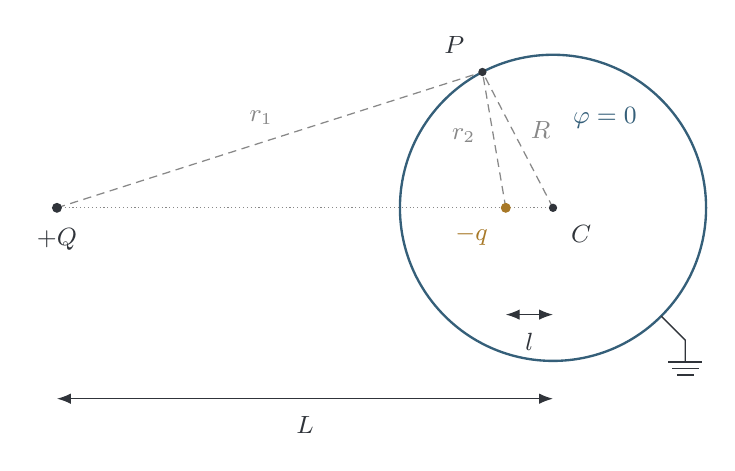
\begin{tikzpicture}[x=1.2cm,y=1.2cm,>=Latex,font=\small,
  meguide/.style={MeTheoryGray,densely dashed,line width=.45pt}]
  \coordinate (MeC) at (1.15,0);
  \coordinate (MeQ) at (-4.1,0);
  \coordinate (MeI) at (0.6501142857,0.0000000000);
  \coordinate (MeP) at (0.4030622400,1.4375270372);
  \draw[MeTheoryBlue,line width=.85pt] (MeC) circle (1.62);
  \draw[meguide] (MeQ)--(MeP) node[pos=.48,above=3pt] {$r_1$};
  \draw[meguide] (MeI)--(MeP) node[pos=.53,left=3pt] {$r_2$};
  \draw[meguide] (MeC)--(MeP) node[pos=.57,right=3pt] {$R$};
  \draw[MeTheoryGray,densely dotted] (MeQ)--(MeC);
  \fill[MeTheoryInk] (MeQ) circle (1.8pt) node[below=4pt] {$+Q$};
  \fill[MeTheoryGold] (MeI) circle (1.8pt) node[below left=3pt] {$-q$};
  \fill[MeTheoryInk] (MeC) circle (1.5pt) node[below right=3pt] {$C$};
  \fill[MeTheoryInk] (MeP) circle (1.5pt) node[above left=3pt] {$P$};
  \node[MeTheoryBlue] at (1.7,.95) {$\varphi=0$};
  \draw[<->,MeTheoryInk,line width=.45pt] (.6501142857,-1.13)--(1.15,-1.13)
    node[midway,below=3pt] {$l$};
  \draw[<->,MeTheoryInk,line width=.45pt] (-4.1,-2.02)--(1.15,-2.02)
    node[midway,below=3pt] {$L$};
  \draw[MeTheoryInk,line width=.5pt] (2.295513,-1.145513)--(2.55,-1.40)--(2.55,-1.63);
  \draw[MeTheoryInk,line width=.5pt] (2.37,-1.63)--(2.73,-1.63)
    (2.41,-1.70)--(2.69,-1.70) (2.46,-1.77)--(2.64,-1.77);
\end{tikzpicture}}

\newcommand{\MeTheoryTwoCylinders}{%
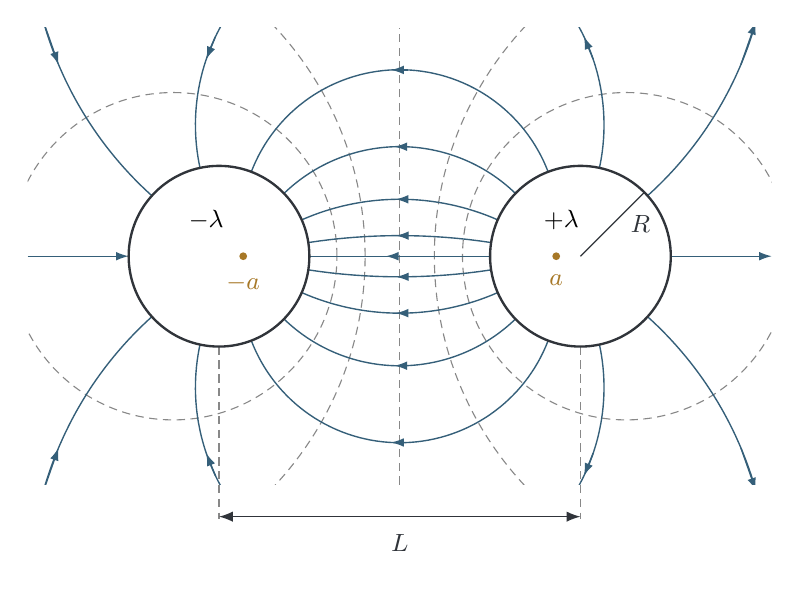
\begin{tikzpicture}[x=1.35cm,y=1.35cm,>=Latex,font=\small,
  mefield/.style={MeTheoryBlue,line width=.5pt},
  mearrow/.style={MeTheoryBlue,line width=.5pt,-{Latex[length=1.6mm,width=1.1mm]}}]
  \begin{scope}
  \clip (-3.5,-2.15) rectangle (3.5,2.15);
  % Equal-potential circles xi=+/- .45,+/- .85; the conductor boundaries are xi=+/-xi0.
  \draw[MeTheoryGray,densely dashed,line width=.4pt] (-2.13038,0.00000) circle (1.539816558);
  \draw[MeTheoryGray,densely dashed,line width=.4pt] (-3.48956,0.00000) circle (3.163787350);
  \draw[MeTheoryGray,densely dashed,line width=.4pt] (3.48956,0.00000) circle (3.163787350);
  \draw[MeTheoryGray,densely dashed,line width=.4pt] (2.13038,0.00000) circle (1.539816558);
  \draw[MeTheoryGray,densely dashed,line width=.4pt] (0,-2.15)--(0,2.15);
  \foreach \mesign in {1,-1}{\begin{scope}[yscale=\mesign]
  % eta=25 degrees; exact bipolar coordinate line.
  \draw[mefield] plot coordinates {(2.33155,0.56890) (2.37667,0.61026) (2.42428,0.65554) (2.47450,0.70520) (2.51394,0.74565) (2.55494,0.78913) (2.59753,0.83593) (2.64173,0.88636) (2.68756,0.94078) (2.73499,0.99958) (2.76750,1.04144) (2.81753,1.10854) (2.85171,1.15640) (2.88651,1.20693) (2.92188,1.26034) (2.95778,1.31680) (2.99412,1.37654) (3.03084,1.43977) (3.04930,1.47277) (3.08637,1.54170) (3.10494,1.57769) (3.14207,1.65290) (3.16058,1.69219) (3.19737,1.77432) (3.21559,1.81724) (3.25154,1.90699) (3.26920,1.95391) (3.28658,2.00224) (3.30366,2.05203) (3.32038,2.10332) (3.33669,2.15617) (3.35254,2.21060) (3.36787,2.26667) (3.38261,2.32443) (3.39670,2.38391) (3.41007,2.44516) (3.42264,2.50823) (3.43431,2.57316) (3.44501,2.64000) (3.45464,2.70877) (3.46309,2.77952) (3.47025,2.85229) (3.47601,2.92710) (3.48025,3.00399) (3.48283,3.08297) (3.48362,3.16408) (3.48246,3.24731) (3.47920,3.33267) (3.47369,3.42017) (3.46574,3.50979) (3.45518,3.60152) (3.44182,3.69530) (3.42547,3.79112) (3.40592,3.88889) (3.38298,3.98856) (3.35642,4.09003) (3.32603,4.19318) (3.29158,4.29791) (3.25286,4.40404) (3.20964,4.51142) (3.16171,4.61985) (3.10883,4.72911) (3.05081,4.83896) (2.98744,4.94911) (2.91854,5.05928) (2.84392,5.16914) (2.76344,5.27833) (2.67697,5.38647) (2.58439,5.49316) (2.48564,5.59798) (2.38068,5.70046) (2.26951,5.80014) (2.15216,5.89655) (2.02873,5.98917) (1.89935,6.07753) (1.76420,6.16111) (1.62352,6.23941) (1.47760,6.31197) (1.32677,6.37831) (1.17143,6.43799) (1.01203,6.49062) (0.84904,6.53581) (0.68300,6.57325) (0.51447,6.60266) (0.34405,6.62383) (0.17234,6.63659) (0.00000,6.64086) (-0.17234,6.63659) (-0.34405,6.62383) (-0.51447,6.60266) (-0.68300,6.57325) (-0.84904,6.53581) (-1.01203,6.49062) (-1.17143,6.43799) (-1.32677,6.37831) (-1.47760,6.31197) (-1.62352,6.23941) (-1.76420,6.16111) (-1.89935,6.07753) (-2.02873,5.98917) (-2.15216,5.89655) (-2.26951,5.80014) (-2.38068,5.70046) (-2.48564,5.59798) (-2.58439,5.49316) (-2.67697,5.38647) (-2.76344,5.27833) (-2.84392,5.16914) (-2.91854,5.05928) (-2.98744,4.94911) (-3.05081,4.83896) (-3.10883,4.72911) (-3.16171,4.61985) (-3.20964,4.51142) (-3.25286,4.40404) (-3.29158,4.29791) (-3.32603,4.19318) (-3.35642,4.09003) (-3.38298,3.98856) (-3.40592,3.88889) (-3.42547,3.79112) (-3.44182,3.69530) (-3.45518,3.60152) (-3.46574,3.50979) (-3.47369,3.42017) (-3.47920,3.33267) (-3.48246,3.24731) (-3.48362,3.16408) (-3.48283,3.08297) (-3.48025,3.00399) (-3.47601,2.92710) (-3.47025,2.85229) (-3.46309,2.77952) (-3.45464,2.70877) (-3.44501,2.64000) (-3.43431,2.57316) (-3.42264,2.50823) (-3.41007,2.44516) (-3.39670,2.38391) (-3.38261,2.32443) (-3.36787,2.26667) (-3.35254,2.21060) (-3.33669,2.15617) (-3.32038,2.10332) (-3.30366,2.05203) (-3.28658,2.00224) (-3.26920,1.95391) (-3.25154,1.90699) (-3.21559,1.81724) (-3.19737,1.77432) (-3.16058,1.69219) (-3.14207,1.65290) (-3.10494,1.57769) (-3.08637,1.54170) (-3.04930,1.47277) (-3.03084,1.43977) (-2.99412,1.37654) (-2.95778,1.31680) (-2.92188,1.26034) (-2.88651,1.20693) (-2.85171,1.15640) (-2.81753,1.10854) (-2.76750,1.04144) (-2.73499,0.99958) (-2.68756,0.94078) (-2.64173,0.88636) (-2.59753,0.83593) (-2.55494,0.78913) (-2.51394,0.74565) (-2.47450,0.70520) (-2.42428,0.65554) (-2.37667,0.61026) (-2.33155,0.56890)};
  \draw[mearrow] (3.20964,1.80303)--(3.35055,2.20359);
  \draw[mearrow] (-3.35055,2.20359)--(-3.20964,1.80303);
  \end{scope}}
  \foreach \mesign in {1,-1}{\begin{scope}[yscale=\mesign]
  % eta=50 degrees; exact bipolar coordinate line.
  \draw[mefield] plot coordinates {(1.87885,0.83097) (1.88855,0.87898) (1.89747,0.93002) (1.90541,0.98428) (1.91212,1.04193) (1.91732,1.10315) (1.92005,1.15151) (1.92159,1.20206) (1.92178,1.25485) (1.92043,1.30994) (1.91734,1.36738) (1.91228,1.42721) (1.90769,1.46843) (1.89880,1.53229) (1.89141,1.57620) (1.87792,1.64406) (1.86718,1.69061) (1.85494,1.73818) (1.84108,1.78674) (1.82552,1.83625) (1.80815,1.88667) (1.78885,1.93795) (1.76751,1.99002) (1.74403,2.04280) (1.71829,2.09622) (1.69019,2.15017) (1.65961,2.20454) (1.62645,2.25922) (1.60887,2.28663) (1.57165,2.34150) (1.55199,2.36892) (1.51051,2.42363) (1.48867,2.45087) (1.44276,2.50503) (1.41867,2.53189) (1.36819,2.58505) (1.34180,2.61129) (1.31463,2.63727) (1.28668,2.66297) (1.25795,2.68835) (1.22844,2.71338) (1.19816,2.73803) (1.16710,2.76228) (1.13528,2.78609) (1.10269,2.80942) (1.06935,2.83226) (1.03527,2.85457) (1.00045,2.87631) (0.96490,2.89746) (0.92865,2.91798) (0.89171,2.93785) (0.85409,2.95703) (0.81581,2.97549) (0.77690,2.99321) (0.73738,3.01015) (0.69726,3.02629) (0.65658,3.04160) (0.61537,3.05606) (0.57364,3.06963) (0.53143,3.08230) (0.48878,3.09404) (0.44570,3.10484) (0.40225,3.11467) (0.35845,3.12351) (0.31434,3.13136) (0.26995,3.13818) (0.22532,3.14398) (0.18050,3.14874) (0.13551,3.15245) (0.09041,3.15511) (0.04523,3.15670) (0.00000,3.15724) (-0.04523,3.15670) (-0.09041,3.15511) (-0.13551,3.15245) (-0.18050,3.14874) (-0.22532,3.14398) (-0.26995,3.13818) (-0.31434,3.13136) (-0.35845,3.12351) (-0.40225,3.11467) (-0.44570,3.10484) (-0.48878,3.09404) (-0.53143,3.08230) (-0.57364,3.06963) (-0.61537,3.05606) (-0.65658,3.04160) (-0.69726,3.02629) (-0.73738,3.01015) (-0.77690,2.99321) (-0.81581,2.97549) (-0.85409,2.95703) (-0.89171,2.93785) (-0.92865,2.91798) (-0.96490,2.89746) (-1.00045,2.87631) (-1.03527,2.85457) (-1.06935,2.83226) (-1.10269,2.80942) (-1.13528,2.78609) (-1.16710,2.76228) (-1.19816,2.73803) (-1.22844,2.71338) (-1.25795,2.68835) (-1.28668,2.66297) (-1.31463,2.63727) (-1.34180,2.61129) (-1.36819,2.58505) (-1.41867,2.53189) (-1.44276,2.50503) (-1.48867,2.45087) (-1.51051,2.42363) (-1.55199,2.36892) (-1.57165,2.34150) (-1.60887,2.28663) (-1.62645,2.25922) (-1.65961,2.20454) (-1.69019,2.15017) (-1.71829,2.09622) (-1.74403,2.04280) (-1.76751,1.99002) (-1.78885,1.93795) (-1.80815,1.88667) (-1.82552,1.83625) (-1.84108,1.78674) (-1.85494,1.73818) (-1.86718,1.69061) (-1.87792,1.64406) (-1.89141,1.57620) (-1.89880,1.53229) (-1.90769,1.46843) (-1.91228,1.42721) (-1.91734,1.36738) (-1.92043,1.30994) (-1.92178,1.25485) (-1.92159,1.20206) (-1.92005,1.15151) (-1.91732,1.10315) (-1.91212,1.04193) (-1.90541,0.98428) (-1.89747,0.93002) (-1.88855,0.87898) (-1.87885,0.83097)};
  \draw[mearrow] (1.81989,1.85310)--(1.73308,2.06604);
  \draw[mearrow] (-1.73308,2.06604)--(-1.81989,1.85310);
  \end{scope}}
  \foreach \mesign in {1,-1}{\begin{scope}[yscale=\mesign]
  % eta=80 degrees; exact bipolar coordinate line.
  \draw[mefield] plot coordinates {(1.39623,0.79386) (1.37572,0.84464) (1.35189,0.89778) (1.32433,0.95317) (1.29820,1.00092) (1.26893,1.04998) (1.24308,1.09005) (1.20748,1.14100) (1.17624,1.18228) (1.14239,1.22388) (1.10582,1.26560) (1.06643,1.30727) (1.02412,1.34867) (0.97882,1.38956) (0.94284,1.41974) (0.89219,1.45913) (0.85219,1.48787) (0.82456,1.50659) (0.79617,1.52490) (0.75218,1.55154) (0.70653,1.57706) (0.65927,1.60133) (0.62690,1.61676) (0.59385,1.63154) (0.54308,1.65242) (0.49094,1.67164) (0.43754,1.68909) (0.38299,1.70466) (0.32741,1.71826) (0.27094,1.72979) (0.21371,1.73920) (0.15589,1.74640) (0.09763,1.75136) (0.03910,1.75404) (0.00000,1.75455) (-0.03910,1.75404) (-0.09763,1.75136) (-0.15589,1.74640) (-0.21371,1.73920) (-0.27094,1.72979) (-0.32741,1.71826) (-0.38299,1.70466) (-0.43754,1.68909) (-0.49094,1.67164) (-0.54308,1.65242) (-0.59385,1.63154) (-0.62690,1.61676) (-0.65927,1.60133) (-0.70653,1.57706) (-0.75218,1.55154) (-0.79617,1.52490) (-0.82456,1.50659) (-0.85219,1.48787) (-0.89219,1.45913) (-0.94284,1.41974) (-0.97882,1.38956) (-1.02412,1.34867) (-1.06643,1.30727) (-1.10582,1.26560) (-1.14239,1.22388) (-1.17624,1.18228) (-1.20748,1.14100) (-1.24308,1.09005) (-1.26893,1.04998) (-1.29820,1.00092) (-1.32433,0.95317) (-1.35189,0.89778) (-1.37572,0.84464) (-1.39623,0.79386)};
  \draw[mearrow] (0.08010,1.75240)--(-0.08010,1.75240);
  \end{scope}}
  \foreach \mesign in {1,-1}{\begin{scope}[yscale=\mesign]
  % eta=110 degrees; exact bipolar coordinate line.
  \draw[mefield] plot coordinates {(1.08880,0.59071) (1.06322,0.61489) (1.03604,0.63942) (1.00718,0.66424) (0.97659,0.68926) (0.94422,0.71438) (0.91699,0.73449) (0.88127,0.75952) (0.85132,0.77940) (0.82014,0.79907) (0.78771,0.81846) (0.75403,0.83749) (0.71912,0.85609) (0.68298,0.87418) (0.65507,0.88736) (0.61682,0.90434) (0.58737,0.91660) (0.54711,0.93224) (0.51621,0.94339) (0.47408,0.95743) (0.44183,0.96728) (0.39802,0.97947) (0.36459,0.98786) (0.33071,0.99557) (0.29641,1.00258) (0.25010,1.01078) (0.21499,1.01606) (0.17959,1.02055) (0.14396,1.02425) (0.10814,1.02714) (0.07217,1.02921) (0.03611,1.03046) (0.00000,1.03088) (-0.03611,1.03046) (-0.07217,1.02921) (-0.10814,1.02714) (-0.14396,1.02425) (-0.17959,1.02055) (-0.21499,1.01606) (-0.25010,1.01078) (-0.29641,1.00258) (-0.33071,0.99557) (-0.36459,0.98786) (-0.39802,0.97947) (-0.44183,0.96728) (-0.47408,0.95743) (-0.51621,0.94339) (-0.54711,0.93224) (-0.58737,0.91660) (-0.61682,0.90434) (-0.65507,0.88736) (-0.68298,0.87418) (-0.71912,0.85609) (-0.75403,0.83749) (-0.78771,0.81846) (-0.82014,0.79907) (-0.85132,0.77940) (-0.88127,0.75952) (-0.91699,0.73449) (-0.94422,0.71438) (-0.97659,0.68926) (-1.00718,0.66424) (-1.03604,0.63942) (-1.06322,0.61489) (-1.08880,0.59071)};
  \draw[mearrow] (0.04935,1.03010)--(-0.04935,1.03010);
  \end{scope}}
  \foreach \mesign in {1,-1}{\begin{scope}[yscale=\mesign]
  % eta=140 degrees; exact bipolar coordinate line.
  \draw[mefield] plot coordinates {(0.92189,0.34213) (0.86627,0.36572) (0.81246,0.38691) (0.75509,0.40781) (0.70110,0.42591) (0.64435,0.44335) (0.59248,0.45789) (0.53081,0.47350) (0.47486,0.48609) (0.41719,0.49754) (0.35798,0.50770) (0.29739,0.51646) (0.23564,0.52370) (0.17295,0.52931) (0.11865,0.53278) (0.05487,0.53520) (0.00000,0.53585) (-0.05487,0.53520) (-0.11865,0.53278) (-0.17295,0.52931) (-0.23564,0.52370) (-0.29739,0.51646) (-0.35798,0.50770) (-0.41719,0.49754) (-0.47486,0.48609) (-0.53081,0.47350) (-0.59248,0.45789) (-0.64435,0.44335) (-0.70110,0.42591) (-0.75509,0.40781) (-0.81246,0.38691) (-0.86627,0.36572) (-0.92189,0.34213)};
  \draw[mearrow] (0.03750,0.53555)--(-0.03750,0.53555);
  \end{scope}}
  \foreach \mesign in {1,-1}{\begin{scope}[yscale=\mesign]
  % eta=165 degrees; exact bipolar coordinate line.
  \draw[mefield] plot coordinates {(0.85977,0.12847) (0.75108,0.14402) (0.64323,0.15734) (0.54024,0.16811) (0.43064,0.17750) (0.32331,0.18463) (0.21217,0.18987) (0.10665,0.19282) (0.00000,0.19382) (-0.10665,0.19282) (-0.21217,0.18987) (-0.32331,0.18463) (-0.43064,0.17750) (-0.54024,0.16811) (-0.64323,0.15734) (-0.75108,0.14402) (-0.85977,0.12847)};
  \draw[mearrow] (0.03369,0.19372)--(-0.03369,0.19372);
  \end{scope}}
  \draw[mefield] (-.85,0)--(.85,0);
  \draw[mearrow] (.13,0)--(-.13,0);
  \draw[mearrow] (2.55,0)--(3.5,0);
  \draw[mearrow] (-3.5,0)--(-2.55,0);
  \end{scope}
  \draw[MeTheoryGray,densely dashed,line width=.4pt] (-1.7,-.85)--(-1.7,-2.47) (1.7,-.85)--(1.7,-2.47);
  \foreach \mec in {-1.7,1.7}{\draw[MeTheoryInk,fill=white,line width=.85pt] (\mec,0) circle (.85);}
  \node at (-1.82,.34) {$-\lambda$};\node at (1.52,.34) {$+\lambda$};
  \fill[MeTheoryGold] (-1.4722431864,0) circle (1.4pt) node[below=3pt] {$-a$};
  \fill[MeTheoryGold] (1.4722431864,0) circle (1.4pt) node[below=3pt] {$a$};
  \draw[MeTheoryInk,line width=.45pt] (1.7,0)--(2.301040764,.601040764) node[midway,right=3pt] {$R$};
  \draw[<->,MeTheoryInk,line width=.45pt] (-1.7,-2.45)--(1.7,-2.45) node[midway,below=3pt] {$L$};
\end{tikzpicture}}

\newcommand{\MeTheoryQuadrupole}{%
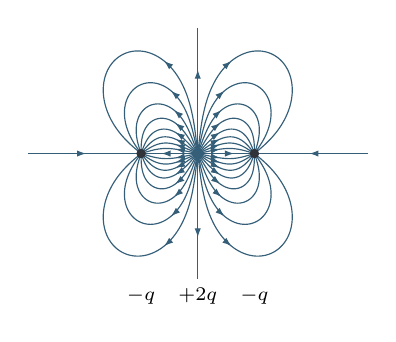
\begin{tikzpicture}[x=.72cm,y=.72cm,>=Latex,font=\scriptsize,
  mefield/.style={MeTheoryBlue,line width=.42pt},
  mearrow/.style={MeTheoryBlue,line width=.42pt,-{Latex[length=1.15mm,width=.8mm]}}]
  \begin{scope}
  \clip (-3,-2.22) rectangle (3,2.22);
  \foreach \mex/\mey in {1/1,-1/1,1/-1,-1/-1}{\begin{scope}[xscale=\mex,yscale=\mey]
  % Exact-field seed polar angle 12.0 degrees, F=1.956292914.
  \draw[mefield] plot coordinates {(0.02934,0.00624) (0.23530,0.04926) (0.30012,0.06170) (0.35924,0.07188) (0.41268,0.07963) (0.46636,0.08552) (0.51424,0.08875) (0.55623,0.08973) (0.60421,0.08851) (0.64608,0.08530) (0.68776,0.08014) (0.73507,0.07203) (0.78199,0.06194) (0.83435,0.04874) (0.89211,0.03251) (0.97223,0.00849)};
  \draw[mearrow] (0.34148,0.06897)--(0.38890,0.07638);
  % Exact-field seed polar angle 24.0 degrees, F=1.827082744.
  \draw[mefield] plot coordinates {(0.02741,0.01220) (0.15397,0.06821) (0.23123,0.10118) (0.29815,0.12772) (0.35473,0.14767) (0.38338,0.15659) (0.41228,0.16461) (0.44146,0.17158) (0.46500,0.17627) (0.48869,0.18008) (0.51252,0.18294) (0.53645,0.18475) (0.56043,0.18546) (0.58443,0.18499) (0.60837,0.18331) (0.63219,0.18041) (0.65583,0.17630) (0.67923,0.17099) (0.70235,0.16455) (0.72514,0.15704) (0.74759,0.14854) (0.76967,0.13916) (0.79679,0.12632) (0.84431,0.10070) (0.90063,0.06629) (0.97580,0.01643)};
  \draw[mearrow] (0.34335,0.14389)--(0.38914,0.15827);
  % Exact-field seed polar angle 36.0 degrees, F=1.618018885.
  \draw[mefield] plot coordinates {(0.02427,0.01763) (0.14625,0.10562) (0.22529,0.16010) (0.26055,0.18291) (0.29126,0.20170) (0.32251,0.21957) (0.34903,0.23359) (0.38150,0.24913) (0.40913,0.26081) (0.43730,0.27112) (0.46599,0.27986) (0.49517,0.28682) (0.51881,0.29094) (0.54863,0.29414) (0.57261,0.29502) (0.60258,0.29390) (0.62642,0.29118) (0.65002,0.28681) (0.67900,0.27909) (0.70164,0.27116) (0.72914,0.25919) (0.75042,0.24810) (0.77605,0.23252) (0.80059,0.21527) (0.82407,0.19660) (0.84653,0.17672) (0.87230,0.15158) (0.89694,0.12534) (0.92068,0.09828) (0.94923,0.06391) (0.98176,0.02317)};
  \draw[mearrow] (0.34369,0.23086)--(0.38698,0.25157);
  % Exact-field seed polar angle 48.0 degrees, F=1.338241257.
  \draw[mefield] plot coordinates {(0.02007,0.02229) (0.13333,0.14692) (0.17454,0.19053) (0.20823,0.22472) (0.24283,0.25798) (0.27860,0.28998) (0.31107,0.31662) (0.33991,0.33817) (0.37484,0.36147) (0.40598,0.37953) (0.43824,0.39549) (0.47160,0.40900) (0.50597,0.41966) (0.53526,0.42610) (0.56499,0.43009) (0.59494,0.43144) (0.61293,0.43092) (0.63087,0.42938) (0.66045,0.42450) (0.68942,0.41675) (0.70639,0.41075) (0.72298,0.40378) (0.74966,0.39009) (0.76503,0.38071) (0.77986,0.37052) (0.80338,0.35190) (0.82952,0.32717) (0.84958,0.30487) (0.87166,0.27645) (0.89170,0.24655) (0.91276,0.21022) (0.93169,0.17273) (0.94886,0.13441) (0.96860,0.08541) (0.99005,0.02762)};
  \draw[mearrow] (0.34974,0.34504)--(0.39027,0.37074);
  % Exact-field seed polar angle 60.0 degrees, F=0.999979761.
  \draw[mefield] plot coordinates {(0.01500,0.02598) (0.07842,0.13532) (0.11829,0.20236) (0.15632,0.26349) (0.18944,0.31353) (0.22434,0.36233) (0.25767,0.40481) (0.29317,0.44549) (0.32680,0.47972) (0.36259,0.51169) (0.38134,0.52668) (0.40067,0.54089) (0.42059,0.55427) (0.44111,0.56673) (0.46220,0.57817) (0.47839,0.58603) (0.50045,0.59548) (0.51733,0.60173) (0.54023,0.60889) (0.55768,0.61331) (0.58124,0.61788) (0.59908,0.62025) (0.61702,0.62169) (0.63501,0.62216) (0.65898,0.62124) (0.67689,0.61937) (0.70053,0.61528) (0.71801,0.61102) (0.73522,0.60574) (0.75763,0.59716) (0.77395,0.58959) (0.79499,0.57806) (0.81017,0.56838) (0.82952,0.55419) (0.84333,0.54265) (0.86077,0.52617) (0.87309,0.51305) (0.88850,0.49465) (0.90272,0.47533) (0.91578,0.45519) (0.92481,0.43963) (0.93587,0.41833) (0.94583,0.39650) (0.95474,0.37421) (0.96264,0.35155) (0.96959,0.32858) (0.97563,0.30536) (0.98201,0.27604) (0.99053,0.22273) (0.99584,0.16900) (0.99887,0.10908) (0.99998,0.02970)};
  \draw[mearrow] (0.35799,0.50784)--(0.39578,0.53742);
  % Exact-field seed polar angle 70.0 degrees, F=0.684023994.
  \draw[mefield] plot coordinates {(0.01026,0.02819) (0.06410,0.17503) (0.10057,0.27029) (0.13490,0.35348) (0.16717,0.42449) (0.19974,0.48869) (0.21722,0.52016) (0.23559,0.55112) (0.25492,0.58149) (0.27182,0.60628) (0.29308,0.63532) (0.31167,0.65887) (0.33507,0.68622) (0.35551,0.70818) (0.37682,0.72929) (0.39903,0.74946) (0.42214,0.76858) (0.44615,0.78655) (0.47107,0.80326) (0.49686,0.81857) (0.52349,0.83237) (0.55092,0.84451) (0.57908,0.85485) (0.60207,0.86173) (0.63129,0.86848) (0.65498,0.87232) (0.67886,0.87471) (0.70284,0.87558) (0.73281,0.87449) (0.76258,0.87090) (0.79195,0.86480) (0.81499,0.85810) (0.83751,0.84983) (0.86477,0.83731) (0.89084,0.82249) (0.91556,0.80550) (0.93425,0.79046) (0.95618,0.77000) (0.97641,0.74786) (0.99490,0.72424) (1.01160,0.69933) (1.02651,0.67330) (1.03964,0.64633) (1.05309,0.61295) (1.06243,0.58444) (1.07013,0.55545) (1.07624,0.52609) (1.08159,0.49049) (1.08446,0.46063) (1.08612,0.42467) (1.08595,0.38868) (1.08407,0.35273) (1.08062,0.31690) (1.07572,0.28124) (1.06951,0.24578) (1.06078,0.20470) (1.05066,0.16394) (1.03938,0.12348) (1.02617,0.08006) (1.00907,0.02729)};
  \draw[mearrow] (0.38119,0.73340)--(0.41744,0.76484);
  % Exact-field seed polar angle 78.0 degrees, F=0.415812653.
  \draw[mefield] plot coordinates {(0.00624,0.02934) (0.05060,0.23501) (0.08075,0.36352) (0.09572,0.42162) (0.11011,0.47367) (0.12554,0.52542) (0.14215,0.57680) (0.16011,0.62772) (0.17956,0.67810) (0.19822,0.72232) (0.21826,0.76593) (0.23979,0.80883) (0.25991,0.84569) (0.28446,0.88694) (0.30736,0.92214) (0.33521,0.96123) (0.36111,0.99429) (0.39249,1.03060) (0.42155,1.06092) (0.45213,1.08971) (0.48422,1.11680) (0.51781,1.14200) (0.55287,1.16511) (0.58935,1.18590) (0.62169,1.20171) (0.66056,1.21760) (0.69475,1.22885) (0.72962,1.23776) (0.76504,1.24418) (0.80083,1.24798) (0.83680,1.24905) (0.86078,1.24819) (0.87872,1.24671) (0.90252,1.24361) (0.92023,1.24043) (0.94362,1.23505) (0.96094,1.23017) (0.98369,1.22253) (1.00045,1.21597) (1.03307,1.20076) (1.04887,1.19213) (1.06934,1.17962) (1.08422,1.16949) (1.10339,1.15505) (1.11723,1.14355) (1.13494,1.12736) (1.14765,1.11461) (1.16379,1.09685) (1.17529,1.08300) (1.18979,1.06388) (1.21284,1.02879) (1.22467,1.00791) (1.23553,0.98651) (1.25220,0.94797) (1.26040,0.92542) (1.26765,0.90254) (1.27812,0.86187) (1.28670,0.81466) (1.29137,0.77293) (1.29361,0.72499) (1.29272,0.67700) (1.28886,0.62917) (1.28221,0.58164) (1.27294,0.53455) (1.26123,0.48800) (1.24532,0.43641) (1.22674,0.38571) (1.20572,0.33597) (1.18247,0.28724) (1.15723,0.23950) (1.13021,0.19275) (1.09842,0.14187) (1.06171,0.08703) (1.01695,0.02358)};
  \draw[mearrow] (0.43447,1.07346)--(0.47028,1.10541);
  % Exact-field seed polar angle 83.5 degrees, F=0.226400401.
  \draw[mefield] plot coordinates {(0.00340,0.02981) (0.03632,0.31028) (0.04885,0.40546) (0.06187,0.49451) (0.07549,0.57740) (0.09085,0.65998) (0.10694,0.73630) (0.12355,0.80636) (0.14368,0.88171) (0.16442,0.95066) (0.18740,1.01889) (0.21059,1.08068) (0.23593,1.14161) (0.26355,1.20155) (0.29356,1.26033) (0.32607,1.31776) (0.36119,1.37363) (0.39900,1.42772) (0.43959,1.47975) (0.47896,1.52503) (0.52069,1.56812) (0.56481,1.60877) (0.58776,1.62809) (0.61131,1.64668) (0.63543,1.66451) (0.66013,1.68154) (0.68539,1.69771) (0.71120,1.71300) (0.75900,1.73812) (0.78625,1.75065) (0.80839,1.75992) (0.83646,1.77050) (0.85921,1.77813) (0.88799,1.78659) (0.91126,1.79246) (0.94061,1.79865) (0.96427,1.80265) (0.99403,1.80643) (1.01795,1.80845) (1.04192,1.80956) (1.06592,1.80974) (1.10188,1.80825) (1.13174,1.80536) (1.16141,1.80095) (1.19082,1.79503) (1.21987,1.78759) (1.24850,1.77863) (1.27662,1.76818) (1.30415,1.75626) (1.33100,1.74290) (1.35712,1.72814) (1.38242,1.71203) (1.41162,1.69098) (1.43491,1.67208) (1.45721,1.65201) (1.47846,1.63085) (1.50254,1.60409) (1.52139,1.58075) (1.54249,1.55160) (1.55881,1.52642) (1.57684,1.49527) (1.59058,1.46860) (1.60551,1.43585) (1.61667,1.40801) (1.62853,1.37402) (1.63716,1.34529) (1.64602,1.31040) (1.65328,1.27514) (1.65897,1.23960) (1.66313,1.20384) (1.66580,1.16794) (1.66702,1.13197) (1.66682,1.09597) (1.66525,1.06001) (1.66235,1.02413) (1.65815,0.98837) (1.65270,0.95279) (1.64604,0.91741) (1.63820,0.88228) (1.62923,0.84742) (1.61915,0.81286) (1.60802,0.77862) (1.59374,0.73913) (1.58043,0.70568) (1.56370,0.66716) (1.54837,0.63458) (1.52938,0.59712) (1.51219,0.56550) (1.49111,0.52917) (1.47220,0.49854) (1.44919,0.46340) (1.42870,0.43381) (1.40393,0.39989) (1.37827,0.36664) (1.35177,0.33406) (1.32448,0.30214) (1.29643,0.27088) (1.26767,0.24026) (1.23826,0.21028) (1.20823,0.18092) (1.17324,0.14807) (1.10594,0.08831) (1.02272,0.01863)};
  \draw[mearrow] (0.55580,1.60085)--(0.59243,1.63186);
  \end{scope}}
  \foreach \mesign in {1,-1}{\begin{scope}[xscale=\mesign]
    \draw[mefield] (.03,0)--(.97,0);\draw[mearrow] (.37,0)--(.64,0);
    \draw[mefield] (1.03,0)--(3,0);\draw[mearrow] (2.28,0)--(1.97,0);
  \end{scope}}
  \foreach \mesign in {1,-1}{\begin{scope}[yscale=\mesign]
    \draw[mefield] (0,.03)--(0,2.22);\draw[mearrow] (0,1.1)--(0,1.48);
  \end{scope}}
  \end{scope}
  \fill[MeTheoryInk] (-1,0) circle (1.7pt);\fill[MeTheoryBlue] (0,0) circle (2pt);\fill[MeTheoryInk] (1,0) circle (1.7pt);
  \node at (-1,-2.52) {$-q$};\node at (0,-2.52) {$+2q$};\node at (1,-2.52) {$-q$};
\end{tikzpicture}}
